\begin{figure}[h!]
    \centering
    \caption{Changes in minimum wage measures in the Chicago-Naperville-Elgin CBSA, July 2019}
    \label{fig:map_mw_chicago_jul2019}

    \begin{subfigure}{0.5\textwidth}
        \centering
        \caption{Residence MW}
        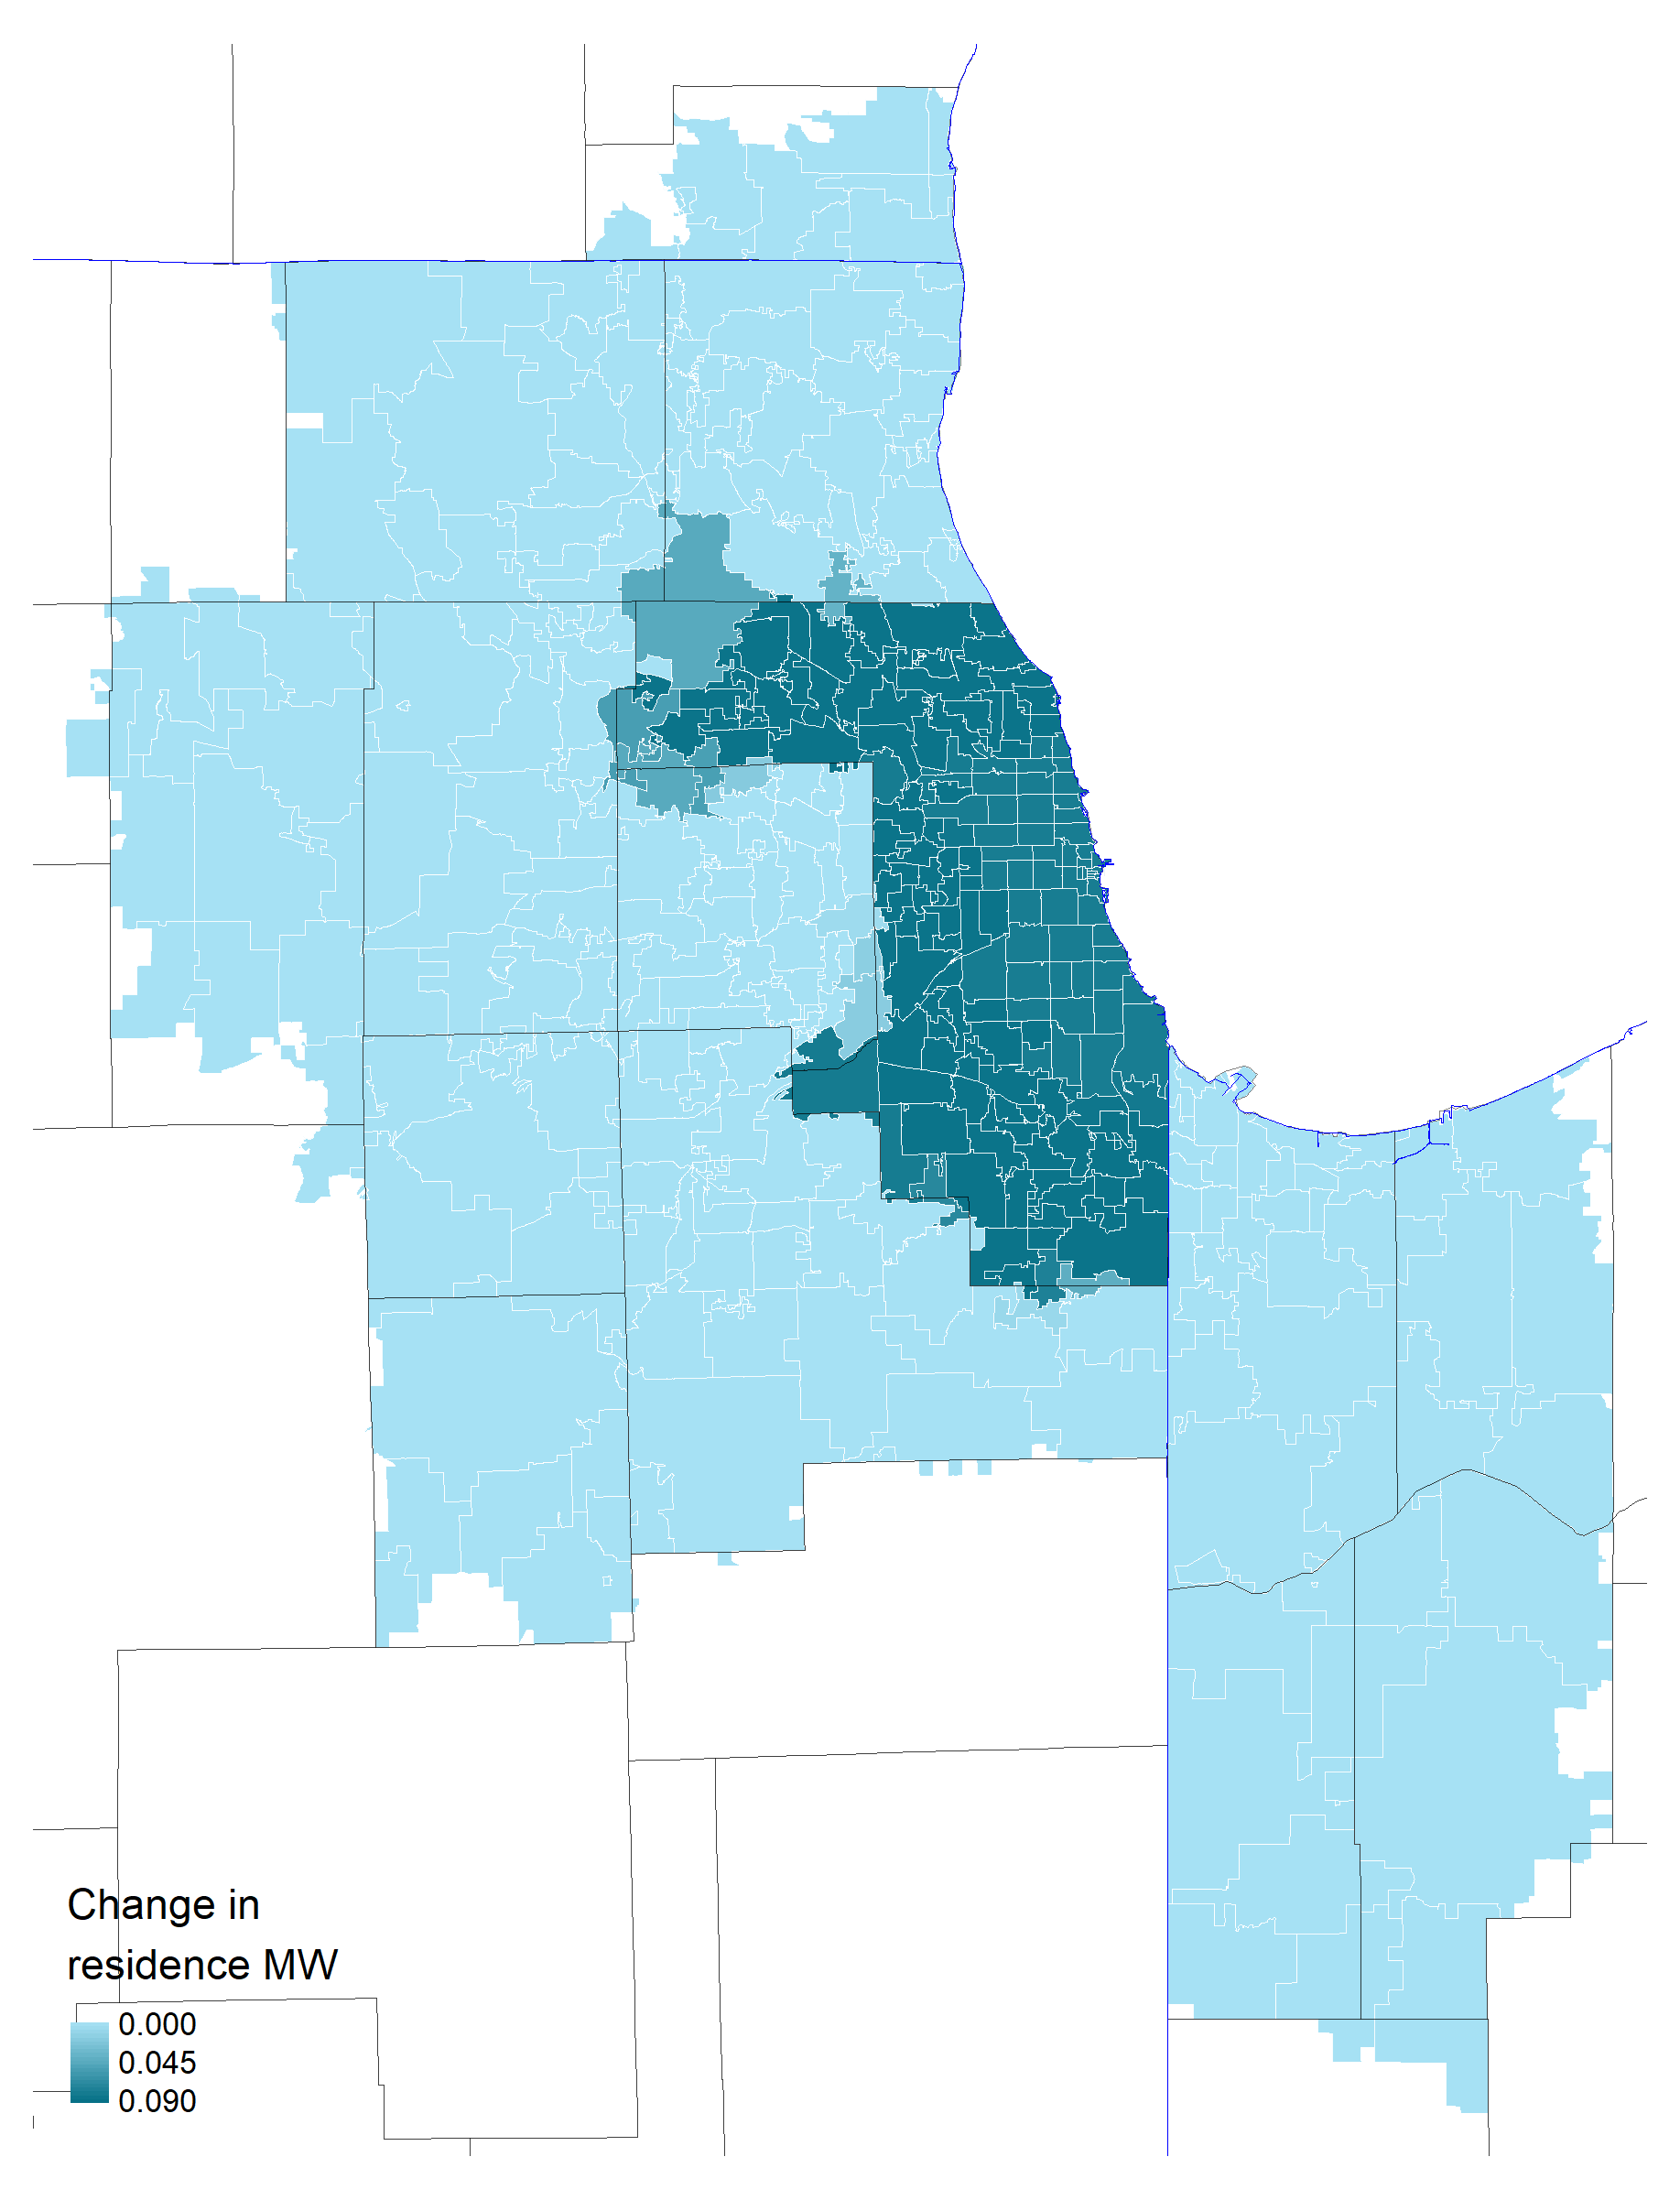
\includegraphics[width = 1\textwidth]
            {maps_events/output/chicago_2019-6_statutory_mw}
    \end{subfigure}%
    \begin{subfigure}{0.5\textwidth}
        \centering
        \caption{Workplace MW}
        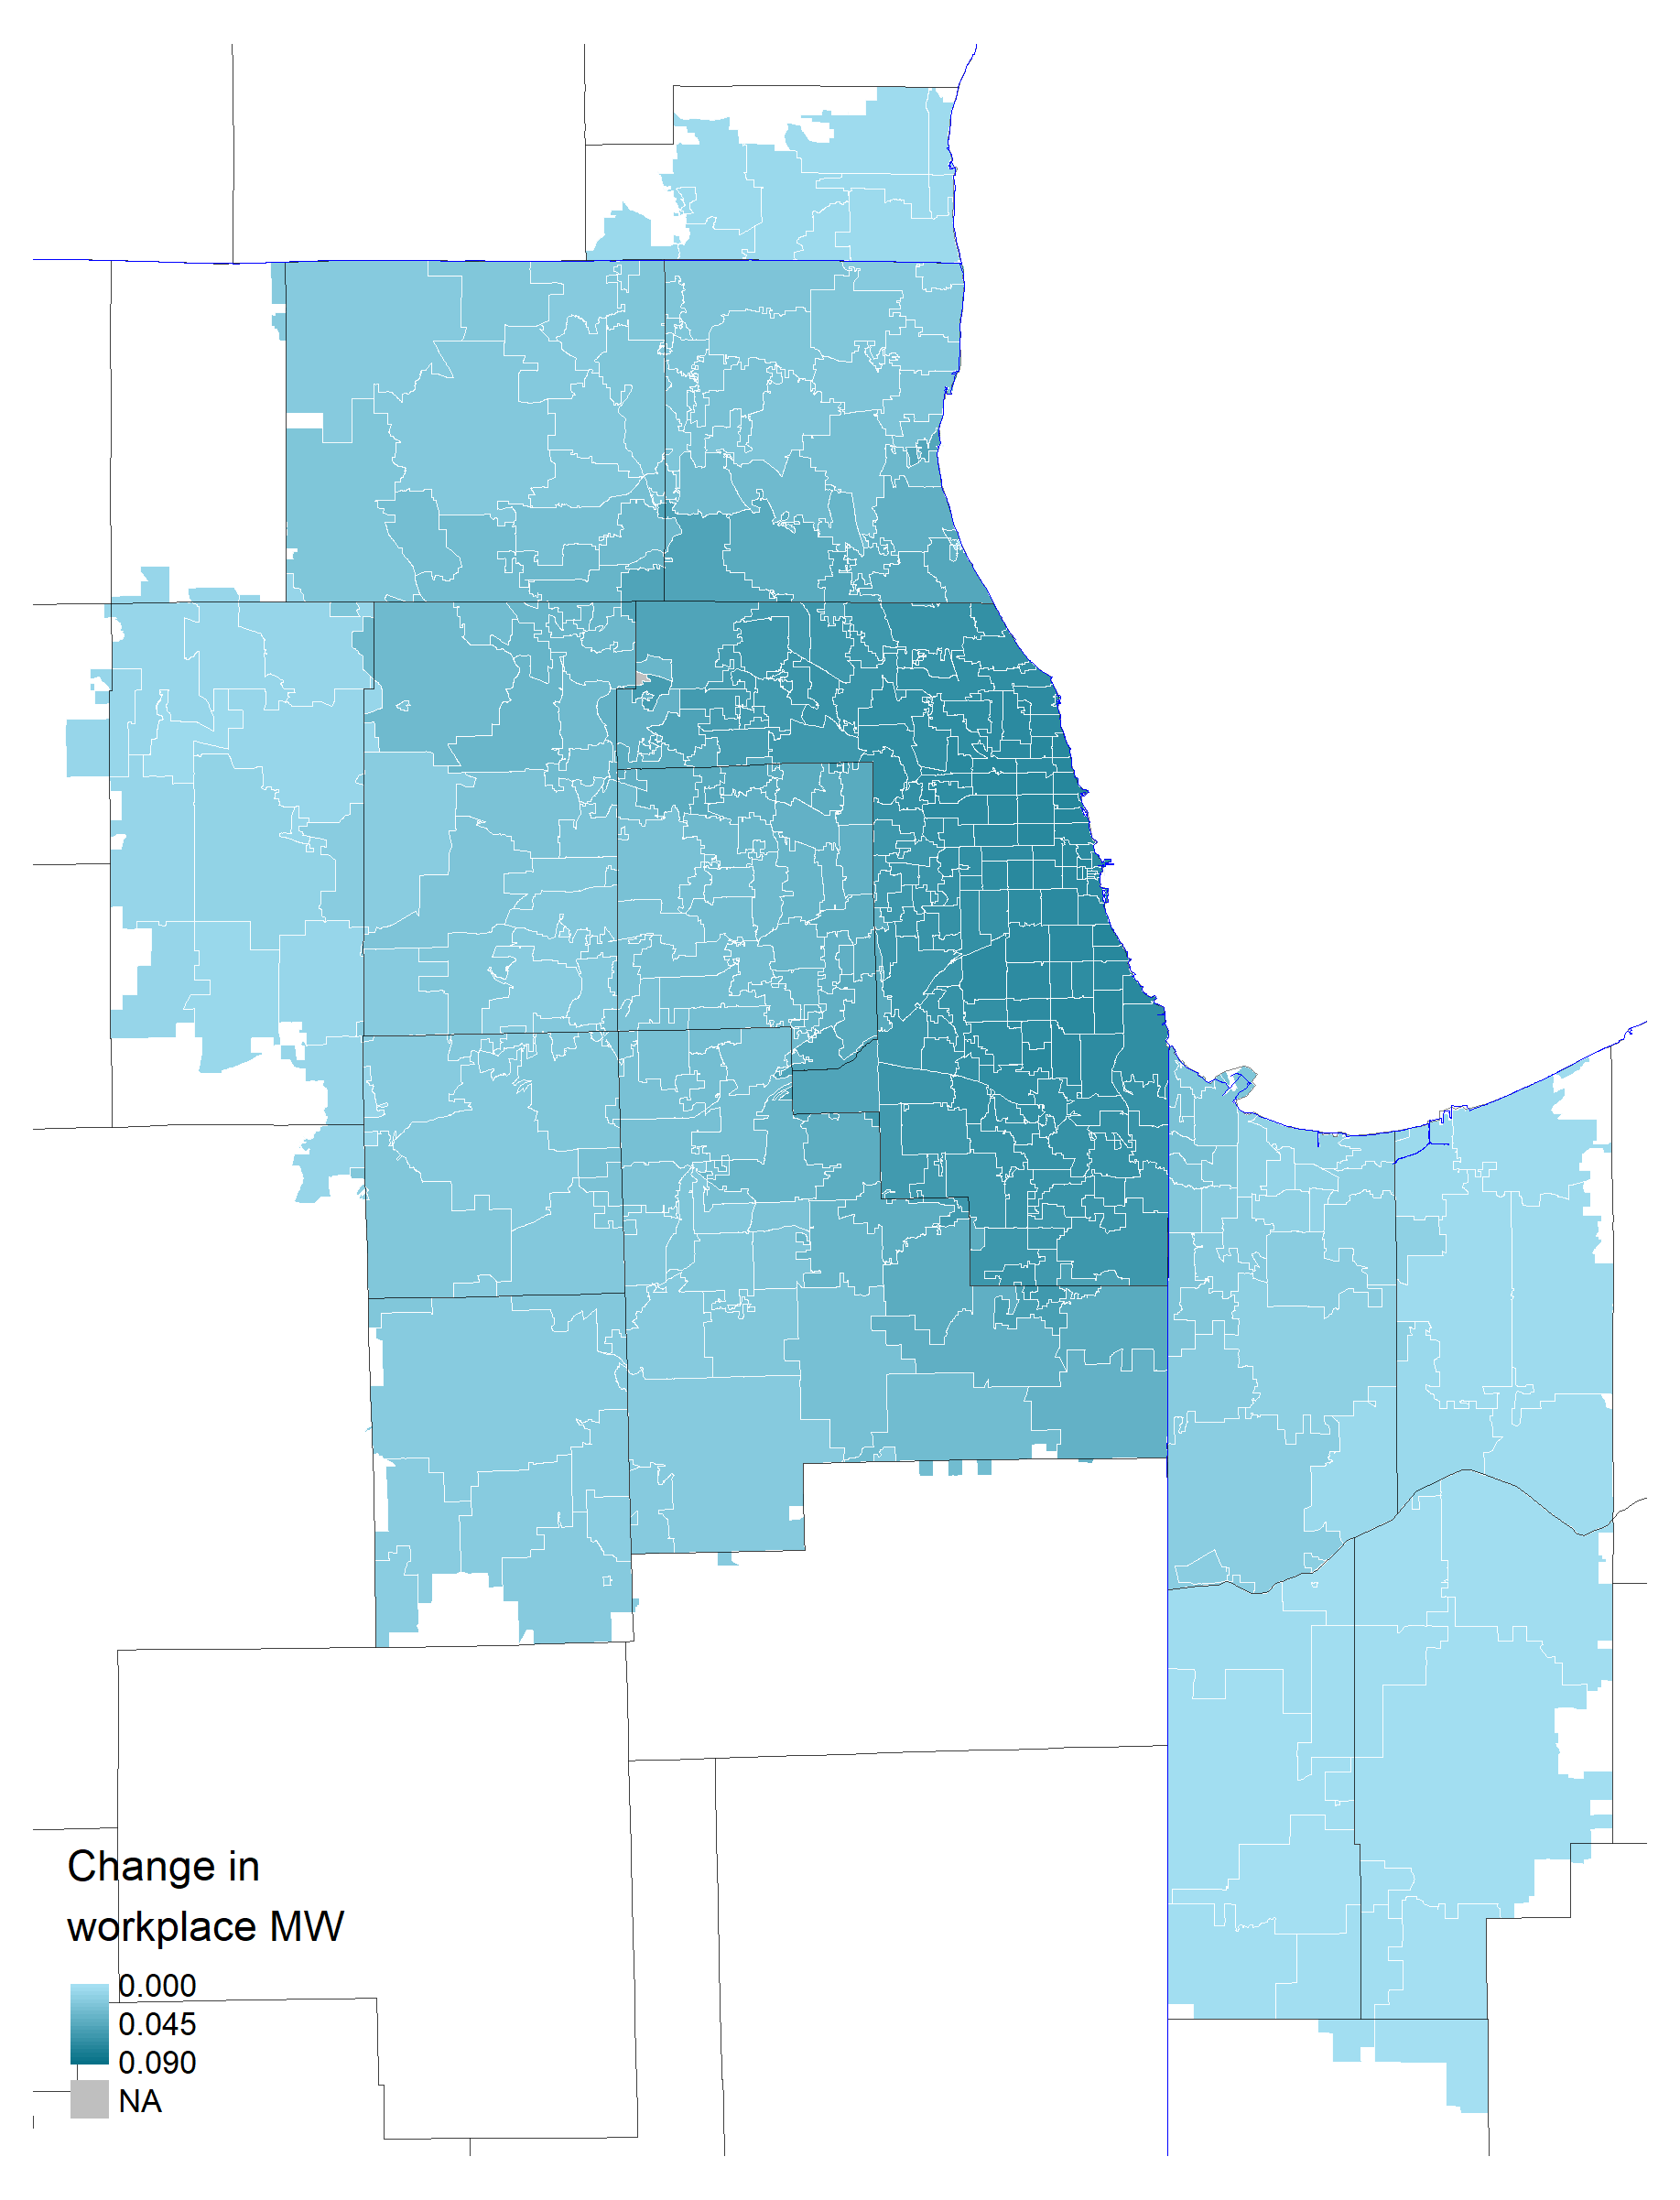
\includegraphics[width = 1\textwidth]
            {maps_events/output/chicago2019-6_wkp_mw}
    \end{subfigure}

    \begin{minipage}{.95\textwidth} \footnotesize
        \vspace{3mm}
        Notes: 
        Data are from the MW panel described in
        Section \ref{sec:data_mw_panel} and from LODES.
        The figure shows the change in 
        the residence MW (panel a) and workplace MW (panel b) 
        in July 2019 in the metropolitan area of Chicago.
        The residence MW is defined as the log of the statutory MW of the given
        ZIP code.
        The workplace MW is defined as the weighted average of the log of the
        statutory MW levels in workplace locations of a ZIP code's residents,
        where weights are given by commuting shares.
    \end{minipage}
\end{figure}
